\section{Introducción}

\IEEEPARstart 
Países como Alemania, España, Japón, Estado Unidos, Italia son las potencias mundiales 
en la generación de energía renovable mediante el uso de energía solar,  este tipo de 
fuente de energía limpia ha adquirido gran importancia en el entorno investigativo en los 
últimos años y han surgido grandes expectativas para el futuro. Según estudios del Ministerio de Minas y 
Energía de Colombia, en el departamento de Nariño hay 15 municipios con 
cobertura eléctrica inferior al 80\% \cite{ministerio_de_minas_y_energia_plan_2008}. Como nueva estratégia para
enfrentar esta problemática se ha planteado la medición y estimación de potenciales energéticos en las zonas más 
viables de la región. Uno de los componentes a analizar es el potencial de biomasa para la generación
eléctrica. Sin embargo, uno de los problemas que se plantea para la ubicación de lugares propicios es la 
ausencia de bases de datos actualizadas en el área de estudio que permitan su respectivo análisis.

Actualmente  la revolución de fuentes energéticas y los cambios acelerados 
 de las condiciones climáticas obliga a las naciones a plantear un cambio a los 
 enfoques de generación de energía, para esta serie de cambios se requiere un 
 análisis de todas y cada una de las fuentes de energía renovables; en algunas 
 situaciones es pertiente resaltar las condiciones para optimizar aprovechamiento del potencial energético. 

``Cada año el sol arroja 4000 veces más energía que la que se consume, lo que demuestra 
que esta fuente energética está aún infravalorada y desaprovechada  en relación a sus 
potenciales energéticos'' \cite{cervantes2014diseno}; 
la implementación para esta fuente energética es posible si un territorio cuenta una buena posición 
geográfica, economía sostenible y fenómenos climáticos regulados, estas condiciones favorables para la energía a base 
de paneles solares o energía térmica se encuentran presentes en muchas regiones de América Central y América del Sur,
 como ventaja adicional la energía solar puede aprovecharse directamente o almacenarse para un consumo posterior
 y no tiene riesgo de agotarse.
 
Esta artículo esta orientado a cumplir con los requerimientos necesarios para la generación de un modelo 
de predicción de energía solar y su extrapolación al resto del área de estudio.

El area de estudio en la investigación fue el departamento de Nariño (Colombia)
el cual esta ubicado en el extremo sur occidental de Colombia, en la frontera con 
Ecuador con una extensión aproximada de 33.268 km, una población de 1,702 millones según
el censo de 2013, su ubicación 
esta en latitud 00° 31' 08'' y 02° 41' 08'' Norte, Longitud 76° 51' 19'' y 79° 01' 34'' Oeste.

\begin{figure}
  \centering
  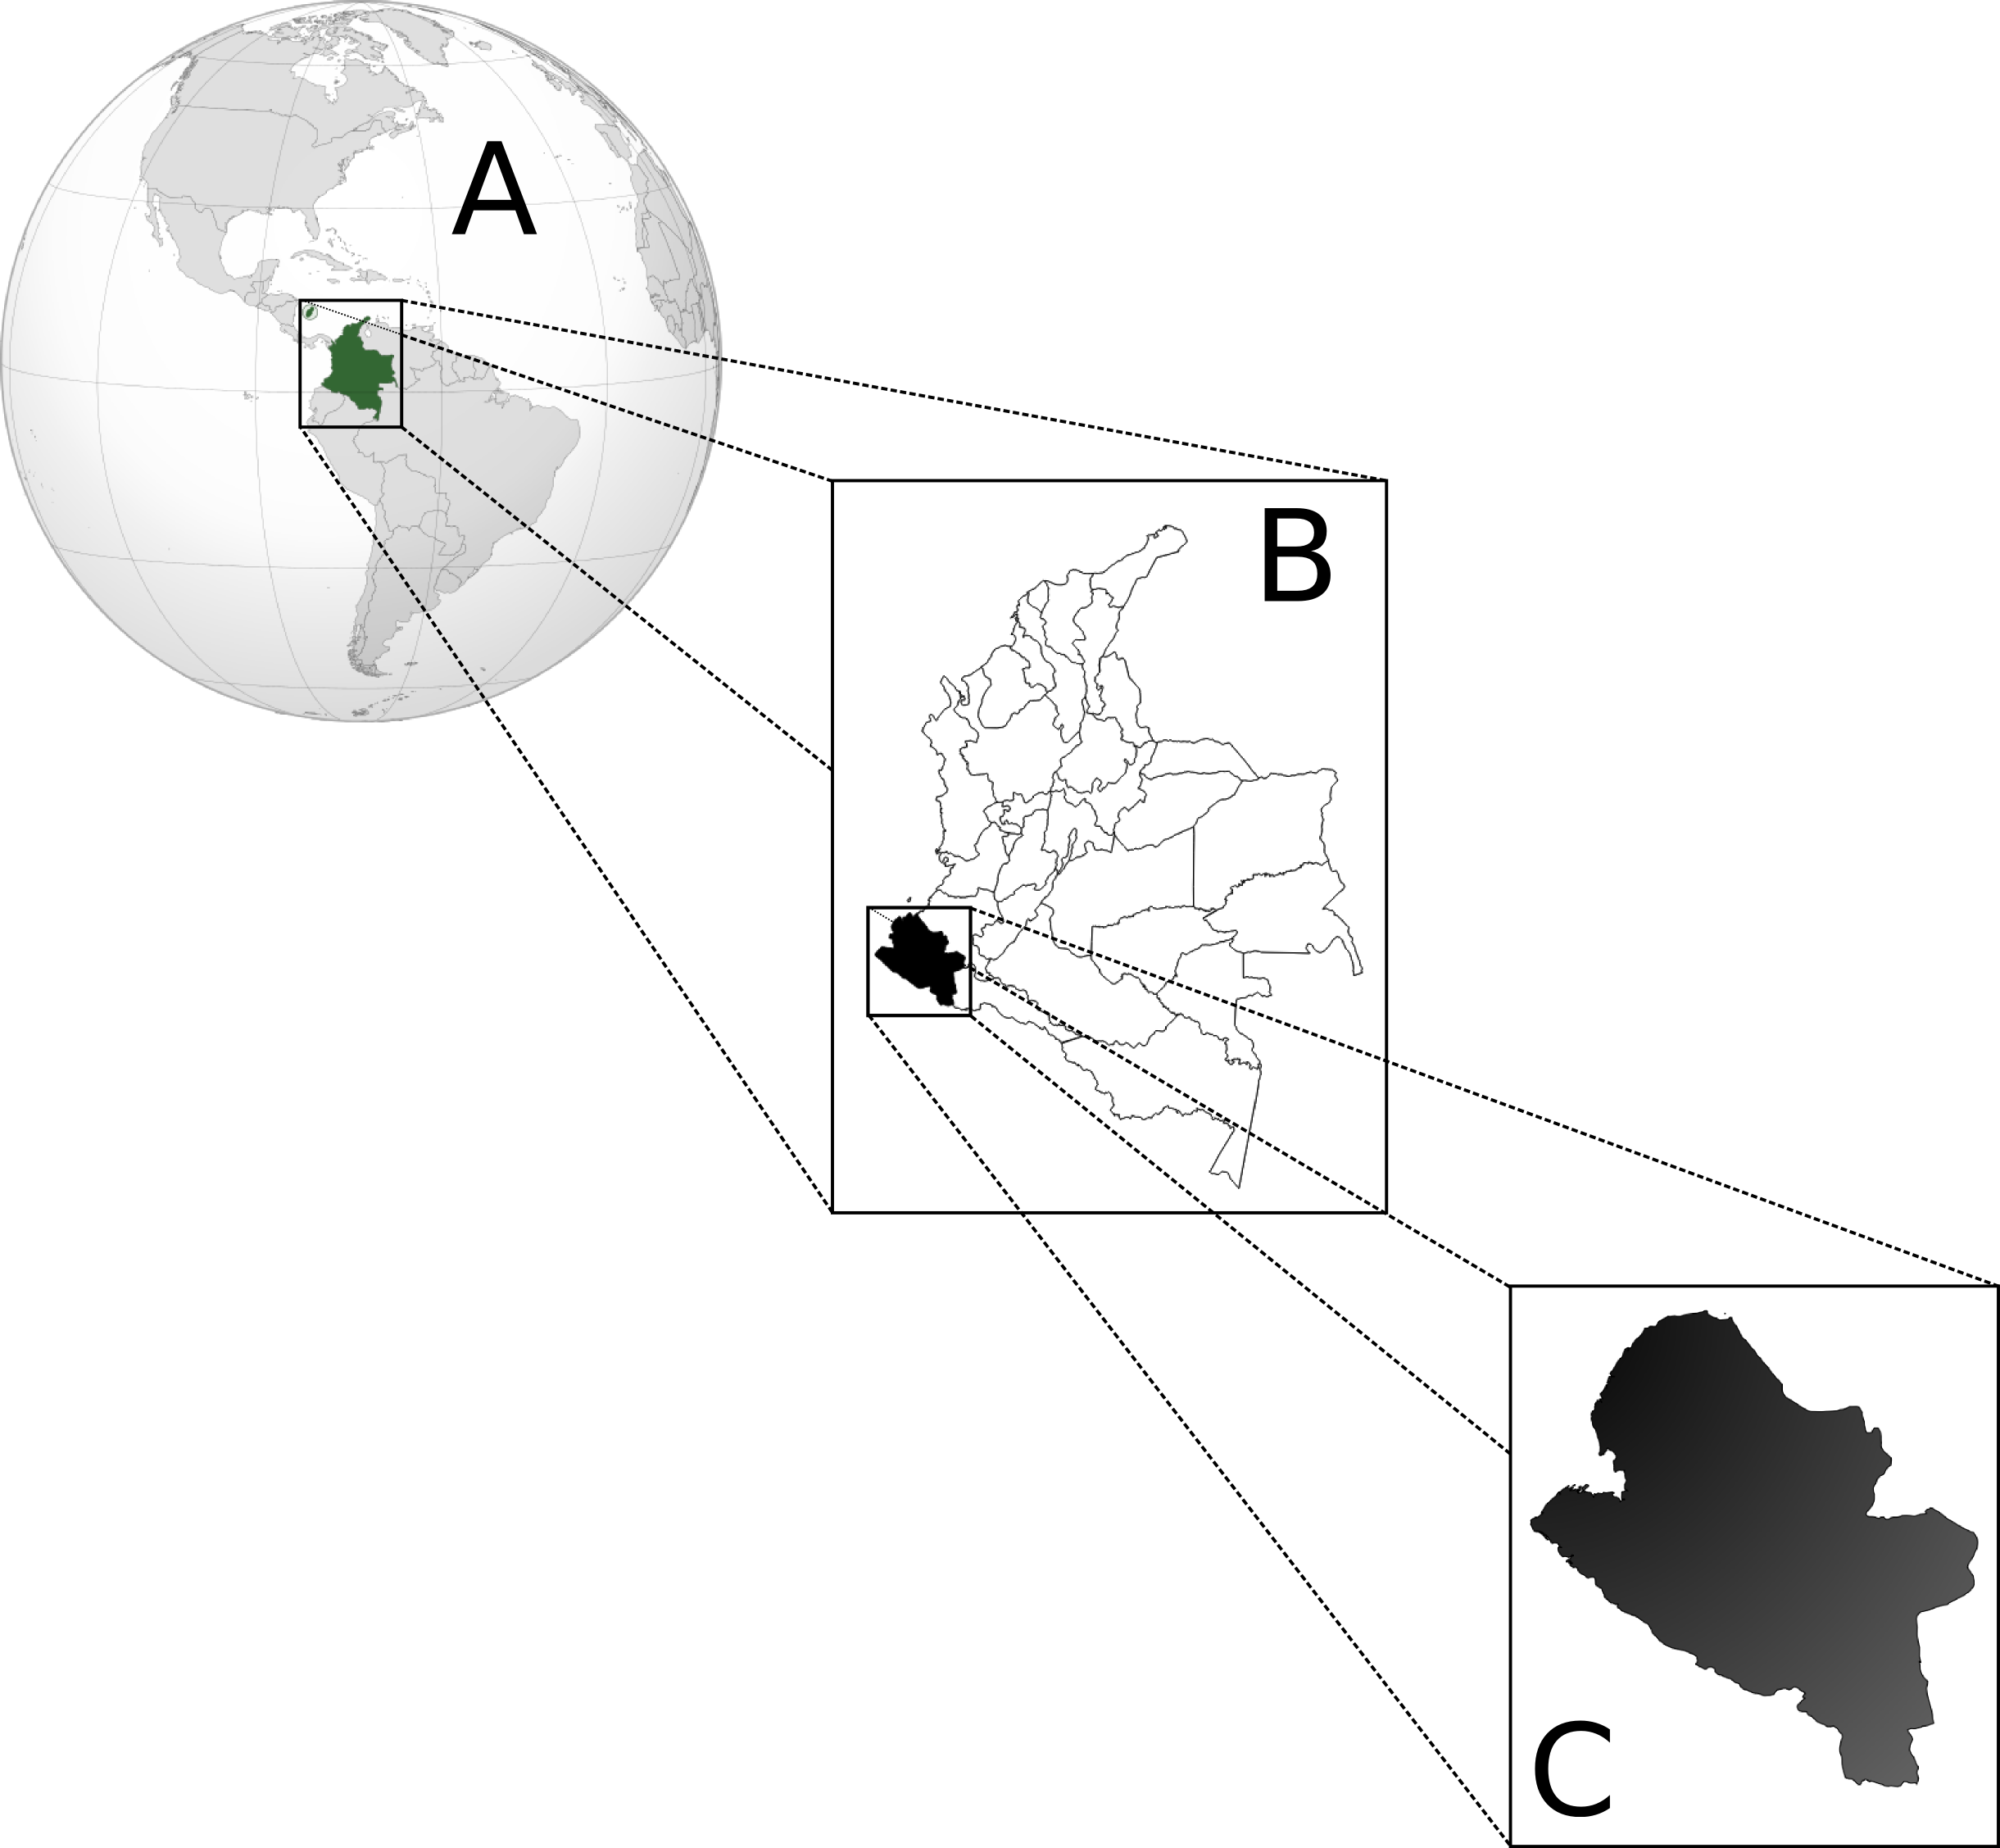
\includegraphics[width = 8cm]{locationNarino.png}
  \caption{Localización area de estudio}
  \label{fig:locationNarino}
\end{figure}